\section{Projektbeskrivelse}
 
\subsection{Problemanalyse}
% Finder beviser for at angry birds ikke er godt for børn.
% 
% 
% 
I det moderne samfund bliver TV og iPads mere og mere inddraget i børns opvækst. Ifølge en undersøgelse af Northwestern University - Center of Human Development\footnote{Northern University; Parenting in the Age of Digital Technology - A national survey; revised 2014}, er 27\% af alle amerikanske familier
% side 8
 \emph{media-centric}, hvilket betyder at disse familier benytter en stor del af deres tid foran en digital skærm af en eller anden form, dette indebærer også deres børn. 

På trods af denne gængse tendens for IT-brug, udviser forældre en generel nervøsitet vedrørende konsekvenserne af børn (under 8 år) forbrug af digitale medier, herunder specielt computerspil. Ifølge undersøgelsen af Northwestern University, er forældre mest af alt nervøse om børns fysiske helbred og sociale evner som konsekvens af meget brug af computerspil på iPads og smart phones.
% side 6 
Selvom videnskaben om konsekvenserne af forbrug af computerspil stadig er ret tvivlsomt og på et tidligt forskningsstadie, er det en relevant problemstilling.

\subsection{Problemformulering}
\emph{Det er et samfundsmæssigt problem at børn har svære ved at socialiserer sig pga. de bruger for lang tid på smartphone apps.}


\subsection{Projektafgrænsning}
For at specificerer en løsning til denne problemstilling tages der udgangspunkt i videospillet Angry Birds af Rovio Entertainment. Ifølge Michael Chorost beskrevet i Psychology today\footnote{Chorost, Michael How I kicked my addiction to the iPhone game Angry Birds; \url{https://www.psychologytoday.com/blog/world-wide-mind/201101/how-i-kicked-my-addiction-the-iphone-game-angry-birds}; 2011}
er der 4 overordnede grunde til at Angry Birds er let at blive afhængig af:
\begin{itemize}
	\item Det er simpelt, ingen "learning curve".
	\item Det er en primitiv nydelse i at destruerer ting.
	\item Selve fysikken i spillet virker realistisk og forudsigeligt.
	\item Det er sjovt. Dyrene i spillet laver backflips og siger sjove lyde.
\end{itemize}

Vi har således tænkt os at udforme en fysisk udgave af et Angry Birds lignende spil, hvor børn kan interagerer socialt ved at spille mod hinanden i stedet for at sidde foran deres iPad. For at omgå copyright kalder vi vores produkt \emph{Moody Feathercreatures}.

Vi har opstillet et overordnet blokdiagram for hvordan vi har tænkt os at efterligne spillet. Se \Cref{fig:blok}.

Vi har valgt at lave et produkt der kan skyde nogle paptårne fra hinanden. Den skal også kunne justerer hastigheden på projektilet afhængigt af projektilets farve (ligesom farverne på fuglene i Angry Birds) og man skal kunne bruge en form for controller til at justere kanonens vinkel i forhold til vandret. Se \Cref{fig:skitse}.

\begin{figure}
	\centering
    \includegraphics[width=13cm]{figures/2_1projektbeskrivelse/blok.png}
	\caption{Blokdiagram af overordnet løsning. Input blokke(røde), Output blokke (gule), Kredse (grønne)}
	\label{fig:blok}
\end{figure}

\begin{figure}
	\centering
    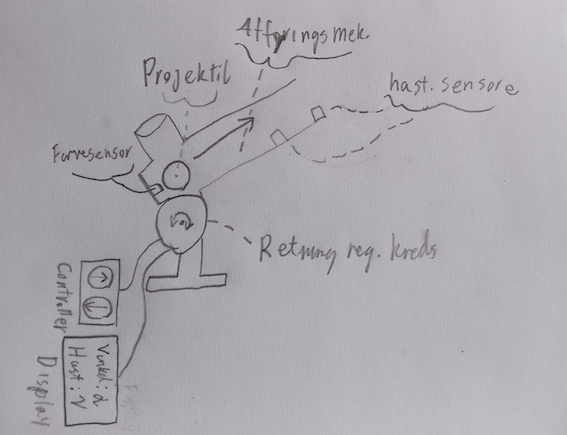
\includegraphics[width=13cm]{figures/2_1projektbeskrivelse/skitse.jpg}
	\caption{En overordnet skitse af produktet}
	\label{fig:skitse}
\end{figure}



Som man kan se på \Cref{fig:blok} er blokkende inddelt således:
\begin{itemize}
	\item Input blokke
	\begin{itemize}
		\item Ladningssensor
		\begin{itemize}
			\item Denne del skal kunne se på farven af et indsat projektil og derfra sende det til arduinoen.
		\end{itemize}
		\item Controller
		\begin{itemize}
			\item Til at bestemme retningen på selve "kanonen".
		\end{itemize}
		\item Hastighedsmåler
		\begin{itemize}
			\item For at kunne måle hastigheden ved udgangen af "kanonen".
		\end{itemize}
	\end{itemize}
	\item Output blokke
	\begin{itemize}
		\item Display
		\begin{itemize}
			\item Til at vise point og hastighed af projektilet. Muligvis andet.
		\end{itemize}
	\end{itemize}
	\item Kredse
	\begin{itemize}
		\item Hastighedsregulerende kreds
		\begin{itemize}
			\item Benyttes til at regulerer hastigheden af projektet afhængigt af dens farve.
		\end{itemize}
		\item Retningsregulerende kreds
		\begin{itemize}
			\item Benyttes til at bestemme retningen alt efter inputtet fra controlleren.
		\end{itemize}
	\end{itemize}
\end{itemize}



\subsection{Overordnede produktkrav}
Da vores produkt er beregnet til børn og unge, skal produktet være sikkert at bruge for børn og unge. Dette betyder at vores "kanon" ikke må skyde hårdt nok, til at volde skade på børn og unge. Derudover skal projektilet "kanonen" skyder, ikke være skarpt eller meget hårdt, da der er risiko for at børnene, ved en fejltagelse, skyder på hinanden. "Kanonen" og projektilet skal være i stand til at vælte papboksene ned. Vi skal sikre os as vores "kanon" og projektil ikke er i strid med den danske våbenlov, og eventuelt udenlandske våbenlove.
Vores produkt skal altså opfylde følgende overordnede produktrav:
\begin{itemize}
\item Sikkert at bruge for børn.
\item Projektilerne skal ikke have en farlig form.
\item Produktet skal skyde hårdt nok til at vælte små papbokse.
\item Produktet skal ikke være i strid med våbenloven.
\end{itemize}



\subsection{Tidsplan for projektet}
\begin{figure}[H]
	\centering
    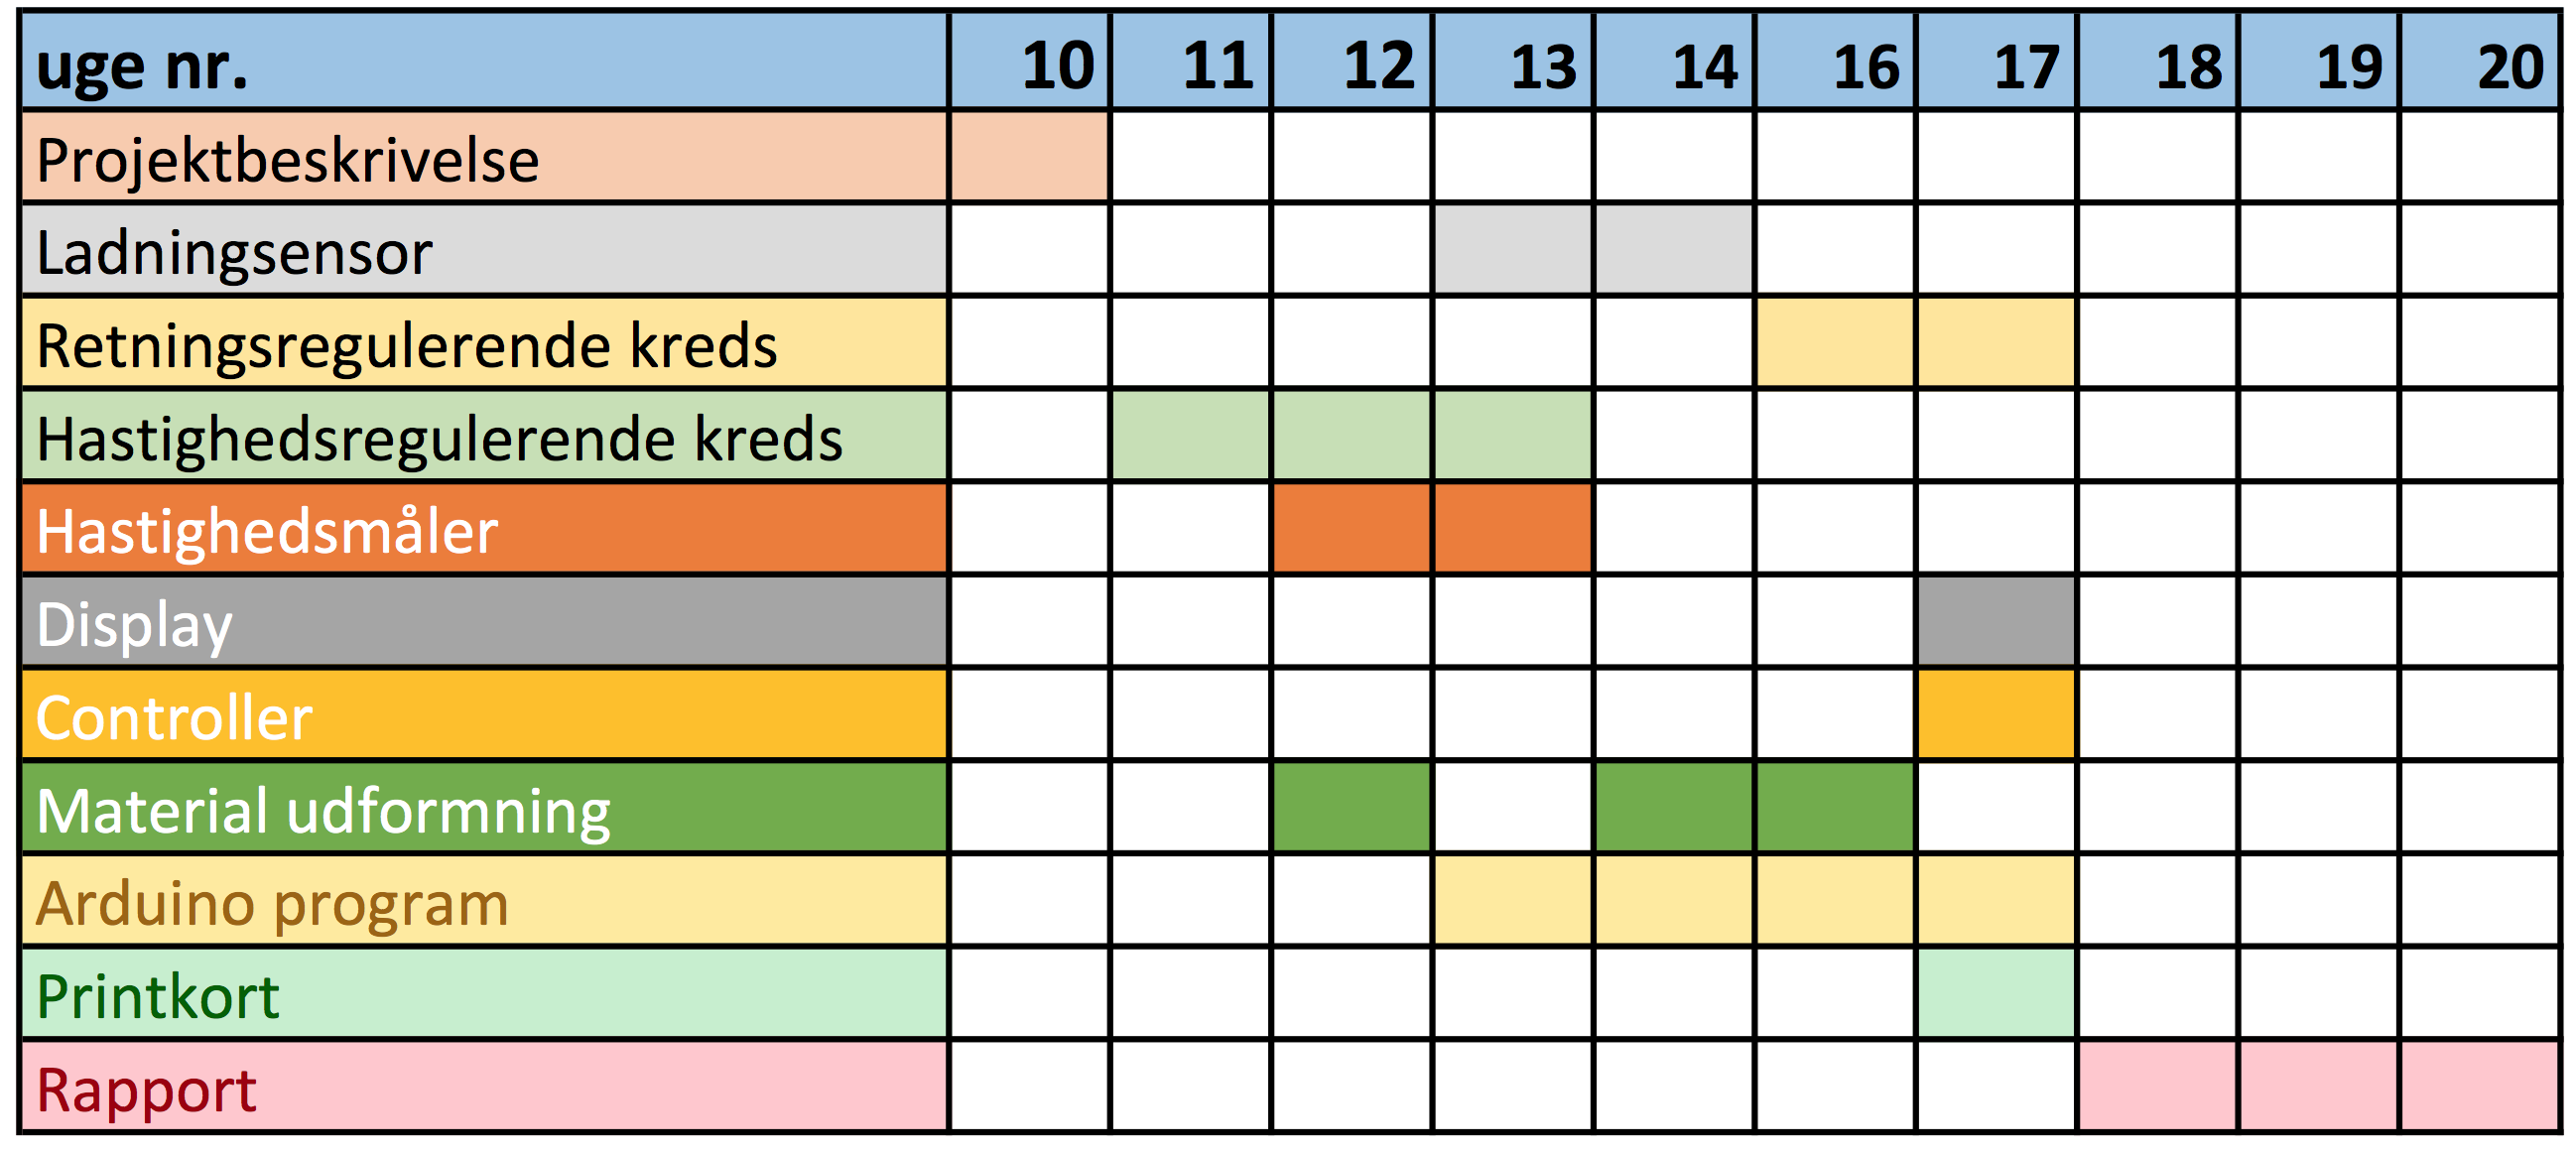
\includegraphics[width=15cm]{figures/2_1projektbeskrivelse/tidsplan.png}
	\caption{Tidsplan}
	\label{fig:tidsplan}
\end{figure}


